% This is part of Analyse Starter CTU
% Copyright (c) 2014
%   Laurent Claessens,Carlotta Donadello
% See the file fdl-1.3.txt for copying conditions.

\begin{exercice}\label{exoDS2012-2-0001}


La figure \ref{graphecos} r\'epresente le graphe de la fonction $f(x)=\cos(x)$, pour $x\in[-\pi,\pi]$. 

\begin{enumerate}
\item Est-ce que la fonction $f(x)=\cos(x)+x^2$ est paire ? Impaire ? P\'eriodique ? Si elle est p\'eriodique, trouver sa p\'eriode. Justifier au mieux vos r\'eponses.
\item Esquissez le graphe des fonctions suivantes pour $x\in[-\pi,\pi]$. 
\end{enumerate}

\begin{multicols}{1}
  \begin{itemize}
    \renewcommand{\labelitemi}{$\bullet$}
  \item $f_1(x)=\cos(2x)$ ;
  \item $f_2(x)=\frac{\cos(x)}{4}$ ;
  \item $f_3(x)=\cos(x)-2$ ;
  \item $f_4(x)=|\cos(x)|$.
  \end{itemize}
\end{multicols}

\begin{figure}[h]
  \begin{center}
     \caption{Le graphe de la fonction cosinus}
   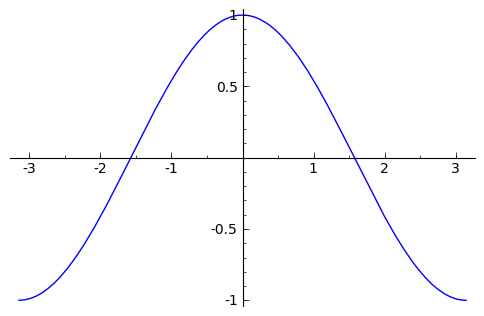
\includegraphics[width=6cm]{pictures_bitmap/cos.png}\label{graphecos}
  \end{center}
 
\end{figure}

\corrref{DS2012-2-0001}
\end{exercice}
